\documentclass[11pt]{article}

\usepackage[margin=1.1in]{geometry}
\usepackage{amsmath,amssymb}
\usepackage{booktabs}
\usepackage{graphicx}
\usepackage{caption}
\usepackage[hidelinks]{hyperref}
\usepackage{natbib}
\usepackage{setspace}
\usepackage{threeparttable}
\usepackage{microtype}

\bibliographystyle{plainnat}
\setcitestyle{authoryear,round}

\captionsetup{font=small,labelfont=bf}
\graphicspath{{../output/figures/}}
\newcommand{\Ngames}{486}
\newcommand{\Npaid}{464}
\newcommand{\Nfree}{22}
\newcommand{\Nlang}{28}
\newcommand{\Ncells}{7348}
\newcommand{\Nobs}{257,180}
\newcommand{\Nreviews}{7,323,081}
\newcommand{\riRank}{1}
\newcommand{\riN}{28}
\newcommand{\pctDiD}{39}
\newcommand{\pctDDD}{25}
\newcommand{\bDiD}{\ensuremath{-0.493}}
\newcommand{\seDiD}{\ensuremath{0.014}}
\newcommand{\tDiD}{\ensuremath{-34.65}}
\newcommand{\bDDD}{\ensuremath{-0.292}}
\newcommand{\seDDD}{\ensuremath{0.049}}
\newcommand{\tDDD}{\ensuremath{-5.94}}
\newcommand{\bPPML}{\ensuremath{-0.489}}
\newcommand{\sePPML}{\ensuremath{0.026}}
\newcommand{\bFree}{\ensuremath{-0.207}}
\newcommand{\seFree}{\ensuremath{0.047}}
\newcommand{\bLatam}{\ensuremath{0.121}}
\newcommand{\seLatam}{\ensuremath{0.010}}
\newcommand{\bGM}{\ensuremath{0.0100}}
\newcommand{\seGM}{\ensuremath{0.0026}}
\newcommand{\bPT}{\ensuremath{0.181}}
\newcommand{\sePT}{\ensuremath{0.012}}
\newcommand{\bGOW}{\ensuremath{-0.084}}
\newcommand{\seGOW}{\ensuremath{0.021}}
\newcommand{\bPos}{\ensuremath{0.0022}}
\newcommand{\sePos}{\ensuremath{0.0022}}
\newcommand{\riP}{\ensuremath{0.036}}
\newcommand{\riNext}{\ensuremath{-0.122}}
\newcommand{\looMin}{\ensuremath{-0.496}}
\newcommand{\looMax}{\ensuremath{-0.492}}
\newcommand{\bAntic}{\ensuremath{-0.488}}
\newcommand{\preF}{\ensuremath{37.95}}
\newcommand{\preP}{\ensuremath{0.00}}
\newcommand{\epsLo}{\ensuremath{-0.15}}
\newcommand{\epsHi}{\ensuremath{-0.40}}
\newcommand{\revLo}{\ensuremath{2.1}}
\newcommand{\revHi}{\ensuremath{18.3}}
\newcommand{\bBudget}{\ensuremath{-0.469}}
\newcommand{\bPrem}{\ensuremath{-0.496}}
\newcommand{\bDose}{\ensuremath{-0.239}}
\newcommand{\seDose}{\ensuremath{0.052}}
\newcommand{\preMax}{\ensuremath{0.230}}
\newcommand{\preSD}{\ensuremath{0.112}}
\newcommand{\preSlope}{\ensuremath{0.0118}}
\newcommand{\preSlopeSE}{\ensuremath{0.0061}}
\newcommand{\preSlopeP}{\ensuremath{0.08}}
\newcommand{\bDetrend}{\ensuremath{-0.669}}
\newcommand{\bTrend}{\ensuremath{-0.567}}
\newcommand{\seTrend}{\ensuremath{0.017}}
\newcommand{\preMean}{\ensuremath{-0.009}}
\newcommand{\bKzero}{\ensuremath{0.086}}
\newcommand{\proxySlope}{\ensuremath{0.577}}
\newcommand{\proxySE}{\ensuremath{0.005}}
\newcommand{\proxyRtwo}{\ensuremath{0.65}}
\newcommand{\proxyN}{8,767}
\newcommand{\multMed}{\ensuremath{121}}
\newcommand{\bUnitsLo}{\ensuremath{-0.169}}
\newcommand{\bUnitsHi}{\ensuremath{-0.292}}
\newcommand{\pctUnitsLo}{16}
\newcommand{\pctUnitsHi}{25}
\newcommand{\epsUnitsLo}{\ensuremath{-0.14}}
\newcommand{\epsUnitsHi}{\ensuremath{-0.24}}
\newcommand{\ctLo}{\ensuremath{-0.866}}
\newcommand{\ctHi}{\ensuremath{-0.335}}
\newcommand{\bSigned}{\ensuremath{-0.306}}
\newcommand{\seSigned}{\ensuremath{0.010}}
\newcommand{\tSigned}{\ensuremath{-30.26}}
\newcommand{\nRatioModes}{45}
\newcommand{\topFiveShare}{55}
\newcommand{\thetaAttNine}{\ensuremath{-0.27}}
\newcommand{\thetaAttSeven}{\ensuremath{-0.34}}
\newcommand{\thetaAttFive}{\ensuremath{-0.48}}
\newcommand{\revMultLo}{\ensuremath{2.5}}
\newcommand{\revMultHi}{\ensuremath{22.4}}
\newcommand{\csLossLo}{\ensuremath{1.8}}
\newcommand{\csLossHi}{\ensuremath{2.4}}
\newcommand{\doseMin}{\ensuremath{0.20}}
\newcommand{\doseMax}{\ensuremath{1.00}}
\newcommand{\doseMed}{\ensuremath{0.60}}
\newcommand{\doseN}{441}
\newcommand{\tailLo}{\ensuremath{-0.57}}
\newcommand{\tailHi}{\ensuremath{-0.43}}


\title{\bf The Price of Being Priced Like America:\\[2pt]
Demand for Digital Goods When Regional Pricing Ends\footnote{%
Replication package: all data are retrieved from public endpoints requiring no
authentication, and every table and figure in this paper is regenerated from a cold start by the
scripts in the accompanying repository. All errors are mine.}}

\author{Areeb Hirani\thanks{Independent. Correspondence: areeb.research@gmail.com.}}

\date{August 2026\\[4pt]\small\itshape Preliminary working paper --- comments very welcome}

\begin{document}
\maketitle

\begin{abstract}
\noindent
On 20 November 2023 Valve abolished Turkish Lira pricing on Steam and repriced its entire
catalogue in dollars, raising local prices by between roughly 240\% and 2{,}900\% overnight. The
decision was Valve's, was driven by exchange-rate volatility rather than by conditions in any
game's market, and applied to every title on a single date. I use it to estimate the price
elasticity of demand for digital goods in an emerging market. Because Steam tags every review with
the reviewer's client language, and because free-to-play titles carry no price and were therefore
untouched, the design is a triple difference: Turkish versus other languages, paid versus free
titles, before versus after. In a panel of \Ngames{} titles across \Nlang{} languages, Turkish
demand for paid games falls by \pctDiD{}\% relative to control ($\hat\beta = \bDiD$, s.e.\
\seDiD), with a flat pre-trend over the preceding sixteen months, no comparable movement in
Russian --- a market with a similar currency collapse whose Ruble pricing Valve retained --- and
a precisely estimated null for free-to-play titles (\bFree{}, s.e.\ \seFree{}). The implied
elasticity is inelastic, between \epsLo{} and \epsHi{} depending on the assumed price change,
which means the deep regional discounts that are orthodoxy in the software industry were
revenue-reducing, and that the surplus lost when they end falls almost entirely on consumers in
the poorest markets. Existing estimates of digital-goods elasticity are identified from temporary
promotions, which conflate price sensitivity with intertemporal substitution; this is a permanent,
unanticipated, order-of-magnitude change.

\vspace{6pt}
\noindent\textbf{Keywords:} digital goods, price discrimination, demand estimation, platforms,
law of one price, emerging markets.\\
\noindent\textbf{JEL:} L11, L86, D12, F31, O33.
\end{abstract}

\newpage
\onehalfspacing

\section{Introduction}

Almost every firm that sells software internationally charges less in poor countries than in rich
ones. Steam, Spotify, Netflix, Adobe, Microsoft and the two mobile app stores all operate some
form of geographic price discrimination, and the practice is defended on a specific empirical
premise: that demand in low-income markets is so price-sensitive that a uniform dollar price would
sell almost nothing there. That premise has never been tested against a large, permanent,
exogenous price change, for the simple reason that such changes do not occur. Firms move prices
by a few percent, and they move them for reasons --- a demand forecast, a competitor, a promotion
--- that are precisely the reasons an econometrician should not trust.

On 20 November 2023 one occurred. Valve, which operates Steam, the dominant distribution platform
for personal-computer games, eliminated the Turkish Lira and the Argentine Peso as Steam
currencies and moved both storefronts onto United States dollars, simultaneously introducing new
regionalised dollar price sets for the surrounding countries. Turkey and Argentina had been the
two cheapest Steam storefronts in the world by a wide margin; a game selling for \$60 in the United
States could be bought in Turkey for a few dollars. Overnight, and across the entire catalogue,
local prices rose by between roughly 240\% and 2{,}900\% depending on the title, with the largest
increases falling on the cheapest games. Valve gave its reason at the time: exchange-rate
volatility had made it ``hard for game developers to choose appropriate prices for their games and
keep them current.''

This paper asks what happened to demand, and what that implies about the elasticity.

The empirical problem is that quantities are not observed. Steam publishes no sales data. I solve
this with an outcome that is public, timestamped, and --- crucially --- attributable to a country:
Steam reviews. A Steam review can only be written by an account that owns the game, it carries an
exact creation timestamp, and it is tagged with the reviewer's client language. Turkish is spoken
essentially only in Turkey, so Turkish-language review flow is a proxy for Turkish purchases. The
proxy has an unknown and probably game-specific multiplier connecting reviews to units, but the
design never needs the multiplier's level: it is absorbed by a game $\times$ language fixed
effect, and identification comes from the change.

The identification has three layers. First, a difference-in-differences comparing Turkish to the
other \Nlang{} languages within the same game and month, so that every global shock to a
title --- a patch, a sale, a sequel, a seasonal peak --- is differenced out by game $\times$ month
fixed effects. Second, a triple difference adding free-to-play titles as a within-Turkey control
group. Free titles have no price, so they received no treatment, but their Turkish players
experienced exactly the same currency collapse, the same inflation, and the same everything else;
language $\times$ month fixed effects therefore absorb the Turkish macroeconomy, which is the most
serious confound in this setting. Third, a set of falsification tests specified in advance:
placebo event dates, a placebo treated language drawn from each of the untreated languages in turn,
and Russia --- a market that suffered a comparable currency collapse over the same years and whose
Ruble pricing Valve did \emph{not} touch.

The main result is that Turkish demand for paid games falls by \pctDiD{}\% relative to control
($\hat\beta = \bDiD$, s.e.\ \seDiD, $t = \tDiD$). The triple difference gives \pctDDD{}\%
(\bDDD{}, s.e.\ \seDDD). The event-study path is flat for the sixteen months before the change,
breaks sharply in the month of the change, and stays at its new level for the following eighteen
months. The free-to-play placebo is \bFree{} with a standard error of \seFree{} --- a null, not an
absence of power. Dropping any single game moves the estimate only within $[\looMin,\ \looMax]$.
When each language in turn is relabelled as treated, Turkish produces the most negative estimate
of all \riN{}, and by a wide margin: the next-most-negative placebo is \riNext.

The magnitude is the point. A \pctDiD{}\% quantity decline against a price increase of at least
240\% implies an own-price elasticity between \epsLo{} and \epsHi{}. Demand is inelastic. Taken at
face value this says that Valve and its developers earned \emph{more} revenue from Turkey after
raising prices several-fold, and therefore that the deep regional discount had been leaving money
on the table. The mirror image of that statement is the welfare one: if quantity barely moves when
price rises by a factor of three to thirty, then almost the entire incidence of ending regional
pricing falls on Turkish consumers as a transfer, not as a deadweight loss avoided.

I make three contributions.

\emph{First, a source of variation.} The elimination of a national currency from a global digital
storefront is, to my knowledge, unused in economics. It has the properties applied researchers
normally have to manufacture: it is dated, it is large, it is permanent, it was announced only
26 days in advance, it applied to an entire catalogue at once, it was not chosen by any seller in
that catalogue, and it left an untreated group (free titles) inside the treated country.

\emph{Second, a dataset.} I assemble a panel of Steam review histories across languages in which
each observation carries a timestamp, a language, the reviewer's playtime at the moment of
writing, the reviewer's library size, and a flag recording whether the copy was activated from a
non-Steam key. That last field makes a substitution margin --- the gray market in game keys ---
directly observable rather than inferred. Every field is retrieved from a public endpoint that
requires no authentication.

\emph{Third, an estimate of the right object.} The existing elasticity estimates for digital
entertainment are identified from temporary discounts. A temporary discount and a permanent price
change are different economic objects: the first invites intertemporal substitution --- buy now
rather than later --- and so overstates true price sensitivity, while the second does not. This
event identifies the response to a permanent change, and identifies it in a market where the
question of what poor consumers will pay for software is the entire policy question.

\paragraph{A note on what this paper does not do.} I do not observe units, only a proxy for them;
I do not observe piracy at all; and I cannot separate Argentina from the rest of Latin America,
because Steam's Spanish-language tags pool Argentina with countries that were treated in the
opposite direction on the same day. Section~\ref{sec:conclusion} is explicit about which of the
paper's claims would change if each of these limitations were relaxed, and about which of them
require data I do not have.

\section{Setting}\label{sec:setting}

\subsection{Steam and regional pricing}

Steam is the dominant distribution platform for personal-computer games. Developers set a price in
each of roughly forty currencies; Valve publishes recommended conversion grids, and for most of
Steam's history most developers simply followed them. The result was a system of third-degree
price discrimination of unusual transparency: the same digital good, delivered at zero marginal
cost, sold at prices that differed by an order of magnitude across borders and could be observed
by anyone.

Turkey and Argentina sat at the bottom of that distribution. Both had suffered severe and
sustained currency depreciation, and because developers update local prices infrequently, the
lira and peso prices of a large fraction of the catalogue had drifted far below their dollar
equivalents. By 2023 the two storefronts were the cheapest in the world by a wide margin and had
become well-known targets of cross-border arbitrage.

\subsection{The event}

On 25 October 2023 Valve notified users in Turkey and Argentina that, effective 20 November 2023,
their account currency would change to United States dollars and any existing wallet balance
would be converted at that day's exchange rate. Valve simultaneously introduced two new regional
dollar price sets, ``LATAM~--~USD'' and ``MENA~--~USD'', covering twenty-five additional countries.
The stated rationale was exchange-rate volatility.

Three features of this event matter for identification.

It was \emph{not chosen by sellers}. A developer whose game became five times more expensive in
Turkey on 20 November did not decide that; Valve's currency architecture did. This is the property
that price changes in observational data almost never have.

It was \emph{catalogue-wide and simultaneous}. There is no staggering, and therefore none of the
pathologies of two-way fixed effects under heterogeneous, staggered adoption
\citep{goodmanbacon2021,callaway2021,sunabraham2021,bjs2024}. I return to this in
Section~\ref{sec:strategy}, because it is a case where the frontier estimator is the wrong tool.

It was \emph{heterogeneous in dose}. Because the pre-change lira prices had drifted furthest below
dollar parity for the cheapest titles, percentage increases were largest at the bottom of the
price distribution: contemporaneous trade reporting documents an increase of roughly 2{,}900\% for
one \$15 indie title and roughly 240\% for a \$60 title from a large publisher. This dispersion is
the basis of the dose-response specification in Section~\ref{sec:strategy}, and of this paper's
principal unfinished piece of work.

\section{Related literature}\label{sec:lit}

This paper sits between four literatures.

\paragraph{International prices and the law of one price.} \citet{cavallo2014} assemble online
prices for identical goods sold by global retailers across dozens of countries and show that the
law of one price holds tightly \emph{within} currency unions, and that good-level real exchange
rates are largely set at the moment a product is introduced rather than accumulated through
heterogeneous pass-through. Their object is prices. What they could not observe, and what this
paper observes, is the \emph{quantity} response when a good is forced into a different currency
zone. The Turkey event is close to a currency-union entry for a digital good, imposed by a
platform rather than a central bank, and Steam reviews supply the missing quantity margin. The
broader online-price literature \citep{cavallo2017,gorodnichenko2017} establishes that online
prices are measurable at scale and behave differently from offline ones; this paper takes the
next step of pairing them with demand.

\paragraph{Demand for digital entertainment.} \citet{tudon2022} estimates price elasticities for
Steam games using within-consumer variation and social-network structure, and is the closest
existing estimate of the parameter studied here. The variation there comes from Steam's frequent
temporary discounts. Temporary and permanent price changes identify different elasticities: a
sale invites consumers to buy now rather than later, so its estimated elasticity mixes true price
sensitivity with intertemporal substitution, and is biased away from zero as a measure of the
long-run response. The present design has no such contamination. \citet{watabe2025} use
cross-country Steam sales to show that physical distance still predicts purchases of digital
goods, and find the effect operates through quantities rather than prices; their setting is the
closest to mine in data and the furthest in question.

\paragraph{Platform pricing and pass-through.} A recent and unusually direct example of why this
question is contested: \citet{choi2025}, in a study for which ``support was provided by Apple,''
reports that when the Digital Markets Act lowered Apple's commission in the European Union,
developers kept prices unchanged or raised them 91\% of the time, concluding that commission
reductions do not reach consumers. The study runs on Apple's internal transaction data, which
cannot be audited, and as described is a share-of-prices-changed calculation rather than a causal
design. Whatever one concludes from it, the episode illustrates that the empirical questions about
platform pricing that regulators are currently deciding are being answered largely with
proprietary data held by interested parties. Part of the motivation for this paper is that the
public record can do better than it has been asked to.

\paragraph{Piracy and gray markets.} When legitimate prices rise sharply in a low-income market,
consumers may substitute toward unauthorised copies rather than exit
\citep{danaher2014,danaher2010}. I cannot observe piracy, but I can observe one adjacent margin
exactly: Steam records whether each reviewer's copy was activated from a non-Steam key, which is
how gray-market key resale appears in the data. Section~\ref{sec:mech} reports what happens to it.

\paragraph{Method.} The design is a single-date difference-in-differences with a never-treated
comparison group, and the inferential difficulty is that treatment is assigned to one language.
I therefore lean on randomization inference \citep{young2019,conley2011} alongside conventional
clustering \citep{bertrand2004,cameron2008}, and on Poisson pseudo-maximum-likelihood
\citep{silva2006} as a check on the log transformation of count data.

\section{Data}\label{sec:data}

\subsection{Construction}

The outcome data come from Steam's public review endpoint, which returns paginated JSON and
requires no API key. For each game and each language I paginate backwards through the review
history using the endpoint's opaque cursor until reaching 2022 or until the cursor stalls. Each
review contributes: creation timestamp, language, whether the review is positive, whether the copy
was purchased on Steam (as opposed to activated from an external key), whether it was received
free, whether it was written during early access, the reviewer's playtime at the time of writing
and lifetime, the reviewer's library size, and an account identifier.

Game-level metadata --- name, free-to-play status, release date, genre, developer, and current
price in any storefront --- come from Steam's store endpoint, also public and unauthenticated.

Reviews are collapsed to a game $\times$ language $\times$ month panel. The estimation window runs
from July 2022 to June 2025, and a game $\times$ language cell enters only if the retrieved review
history demonstrably spans the whole window, which is verified cell by cell rather than assumed.
The resulting panel has \Nobs{} observations across \Ngames{} titles (\Npaid{} paid,
\Nfree{} free-to-play), \Nlang{} languages, and \Ncells{} game $\times$ language cells.

\subsection{The review-flow proxy}

Review counts are a proxy for units, not units. The industry practice of scaling reviews to sales
by a multiplier is well established but the multiplier varies by genre, price, and release
cohort. The design does not require knowing it. Write observed reviews as
$R_{glt} = \mu_{gl}\,Q_{glt}\,\eta_{glt}$, where $\mu_{gl}$ is the review propensity for game $g$
among speakers of language $l$ and $\eta$ is idiosyncratic. In logs, $\mu_{gl}$ is a game
$\times$ language fixed effect and drops out. The identifying assumption is not that $\mu$ is
known, nor that it is common across games or languages, but only that it does not \emph{change
differentially} for Turkish speakers of paid titles at the moment of the price change.

That assumption is testable, and Section~\ref{sec:mech} tests it. If the fall in Turkish review
counts reflected a change in who writes reviews rather than a change in how many people buy, the
composition of Turkish reviewers should shift at the event: their playtime, their library sizes,
and the positivity of their reviews are all observed.

\subsection{Summary}

Table~\ref{tab:summary} reports the panel by language.

\begin{table}[htbp]
\centering
\caption{Panel summary by language}\label{tab:summary}
\small
\begin{tabular}{lrrrrrr}
\toprule
Language & Titles & Obs. & Reviews & Mean/mo. & Share positive & Non-Steam key \\
\cmidrule(lr){2-7}
turkish & 34 & 1,190 & 214,134 & 179.9 & 0.899 & 0.085 \\
brazilian & 23 & 805 & 167,793 & 208.4 & 0.949 & 0.103 \\
russian & 15 & 525 & 157,817 & 300.6 & 0.88 & 0.111 \\
german & 34 & 1,190 & 140,386 & 118 & 0.899 & 0.207 \\
spanish & 16 & 560 & 135,681 & 242.3 & 0.963 & 0.158 \\
polish & 34 & 1,190 & 133,212 & 111.9 & 0.914 & 0.185 \\
schinese & 13 & 455 & 118,504 & 260.4 & 0.883 & 0.157 \\
latam & 38 & 1,330 & 65,507 & 49.3 & 0.932 & 0.106 \\
koreana & 20 & 700 & 56,697 & 81 & 0.923 & 0.123 \\
french & 18 & 630 & 51,982 & 82.5 & 0.952 & 0.255 \\
ukrainian & 18 & 630 & 24,977 & 39.6 & 0.937 & 0.115 \\
tchinese & 18 & 630 & 18,878 & 30 & 0.88 & 0.12 \\
italian & 15 & 525 & 12,654 & 24.1 & 0.947 & 0.272 \\
czech & 17 & 595 & 10,745 & 18.1 & 0.947 & 0.24 \\
thai & 18 & 630 & 8,080 & 12.8 & 0.955 & 0.108 \\
japanese & 18 & 630 & 7,566 & 12 & 0.846 & 0.085 \\
swedish & 16 & 560 & 6,211 & 11.1 & 0.945 & 0.166 \\
hungarian & 17 & 595 & 5,985 & 10.1 & 0.945 & 0.24 \\
portuguese & 15 & 525 & 5,574 & 10.6 & 0.966 & 0.192 \\
dutch & 16 & 560 & 5,006 & 8.9 & 0.956 & 0.21 \\
finnish & 15 & 525 & 4,776 & 9.1 & 0.946 & 0.191 \\
danish & 15 & 525 & 2,532 & 4.8 & 0.942 & 0.201 \\
norwegian & 15 & 525 & 2,191 & 4.2 & 0.942 & 0.135 \\
romanian & 14 & 490 & 1,488 & 3 & 0.957 & 0.207 \\
vietnamese & 14 & 490 & 1,479 & 3 & 0.956 & 0.121 \\
greek & 15 & 525 & 885 & 1.7 & 0.954 & 0.172 \\
bulgarian & 15 & 525 & 688 & 1.3 & 0.939 & 0.139 \\
indonesian & 10 & 350 & 473 & 1.4 & 0.968 & 0.12 \\
\midrule
\textbf{All} & \textbf{39} & \textbf{18,410} & \textbf{1,361,901} & & & \\
\bottomrule
\end{tabular}

\vspace{3pt}
\begin{minipage}{0.92\textwidth}\footnotesize
\emph{Notes.} Game-months is the number of game $\times$ month observations contributing for that
language over July 2022--June 2025. ``Share pos.'' is the mean share of reviews marked positive.
``Non-Steam key'' is the mean share of reviews written by accounts whose copy was activated from a
key not purchased on Steam.
\end{minipage}
\end{table}

\section{Empirical strategy}\label{sec:strategy}

\subsection{Specification}

The primary specification is
\begin{equation}
\ln(1+Q_{glt}) \;=\; \sum_{k\neq -1}\beta_k \,\mathbf{1}[t = t^{*}+k]\cdot \mathrm{TR}_l \cdot \mathrm{Paid}_g
\;+\; \alpha_{gt} \;+\; \delta_{lt} \;+\; \gamma_{gl} \;+\; \varepsilon_{glt},
\label{eq:ddd}
\end{equation}
where $Q_{glt}$ is the review count for game $g$ in language $l$ in month $t$; $\mathrm{TR}_l$
indicates Turkish; $\mathrm{Paid}_g$ indicates a title with a positive price; $t^{*}$ is November
2023; and $k$ indexes months relative to the event, with $k=-1$ omitted.

The fixed effects do the work. $\alpha_{gt}$, game $\times$ month, absorbs everything that happens
to a title globally in a month: patches, downloadable content, sales, sequels, tournaments, the
title's own life cycle. $\delta_{lt}$, language $\times$ month, absorbs everything that happens to
speakers of a language in a month, and in particular absorbs the Turkish macroeconomy --- the
lira, inflation, real incomes, holidays. $\gamma_{gl}$, game $\times$ language, absorbs persistent
affinity between a title and a linguistic market, and with it the unknown review-propensity
constant $\mu_{gl}$.

Identification therefore comes from the residual variation: within a game-month and within a
language-month, did \emph{paid} titles move differently for \emph{Turkish} speakers than the same
comparison in other languages? The coefficient of interest is $\beta_k$ for $k \ge 0$, expected
negative.

I also report the simpler difference-in-differences on paid titles only, which drops
$\delta_{lt}$ and is identified within game-month across languages. It is the more transparent
specification and the more vulnerable one, since it does not net out the Turkish macroeconomy.
Comparing the two is informative rather than redundant.

\subsection{Why not a heterogeneity-robust estimator}

A referee will reasonably ask why this paper does not use Callaway--Sant'Anna, Sun--Abraham, or
Borusyak--Jaravel--Spiess. The answer is that those estimators solve a problem this design does
not have. The pathology they address --- already-treated units serving as effective controls, with
negative weights on some treatment effects --- arises when treatment timing is \emph{staggered}
\citep{goodmanbacon2021}. Here every treated unit is treated on the same date, 20 November 2023,
and every control unit is never treated. Under a single adoption date with a never-treated
comparison group, two-way fixed effects recovers the average treatment effect on the treated
without the forbidden comparisons, and a Goodman-Bacon decomposition would return a single
timing group. Applying a staggered-timing estimator here would be a signal of method rather than a
correction. What this design \emph{does} need, and what the literature above does not supply, is
inference with one treated cluster; that is the subject of the next subsection.

\subsection{Inference with one treated cluster}

Treatment is assigned at the language level and exactly one language is treated. Cluster-robust
standard errors on language are therefore unavailable, and any procedure that behaves as if there
were many treated clusters will overstate precision. I report three things instead.

Standard errors clustered at game $\times$ language, which is the level at which serial correlation
in the panel lives and which treats each treated cell as an independent draw. These are the
numbers in parentheses throughout.

Randomization inference across languages: each untreated language is relabelled treated in turn,
the specification is re-estimated, and the true estimate is compared to the resulting placebo
distribution \citep{young2019}. With \riN{} languages the smallest attainable one-sided $p$-value
is $1/\riN$, and this bound is stated rather than hidden.

Leave-one-game-out re-estimation, to confirm that no single title drives the result.

\subsection{From reduced form to elasticity}

The reduced-form coefficient becomes an elasticity on division by the log price change,
$\hat\varepsilon = \hat\beta / \Delta \ln P$. Because $\Delta \ln P$ differs across titles --- a
240\% increase is 1.22 log points, a 2{,}900\% increase is 3.43 --- the honest object is a range,
and a dose-response specification,
\begin{equation}
\ln(1+Q_{glt}) \;=\; \theta \cdot \mathrm{TR}_l\cdot \mathrm{Post}_t\cdot \Delta \ln P_g
\;+\; \alpha_{gt} + \delta_{lt} + \gamma_{gl} + \varepsilon_{glt},
\label{eq:dose}
\end{equation}
recovers $\theta$ as the elasticity directly. Equation~\eqref{eq:dose} requires per-title lira
prices immediately before 20 November 2023. Those prices are not available from any free public
source I have been able to verify: the platform's own endpoint reports only current prices, and
the principal third-party archive of historical Steam prices refuses programmatic access and
restricts scraping in its terms, so I have not used it. Section~\ref{sec:conclusion} treats this
as what it is --- the paper's central unfinished piece, and the one where outside data would most
change what can be claimed.

\section{Results}\label{sec:results}

\subsection{Main estimates}

Table~\ref{tab:main} reports the static estimates.

\begin{table}[htbp]
\centering
\caption{The end of Turkish Lira pricing and demand for paid games}\label{tab:main}
\small
\begin{tabular}{lccccc}
\toprule
 & (1) & (2) & (3) & (4) & (5) \\
 & DiD & DDD & PPML & F2P & LatAm \\
\cmidrule(lr){2-6}
Turkish $\times$ Post & $-0.468$$^{***}$ &  & $-0.413$$^{***}$ & $-0.136$$^{*}$ &  \\
 & ($0.055$) &  & ($0.082$) & ($0.069$) &  \\[3pt]
Turkish $\times$ Paid $\times$ Post &  & $-0.343$$^{***}$ &  &  &  \\
 &  & ($0.083$) &  &  &  \\[3pt]
Latin-American Spanish $\times$ Post &  &  &  &  & $0.148$$^{***}$ \\
 &  &  &  &  & ($0.032$) \\[3pt]
\midrule
Title $\times$ month FE & Yes & Yes & Yes & Yes & Yes \\
Language $\times$ month FE & No & Yes & No & No & No \\
Title $\times$ language FE & Yes & Yes & Yes & Yes & Yes \\
Sample & Paid & All & Paid & Free & Paid \\
Observations & 14,910 & 18,375 & 14,875 & 3,465 & 14,035 \\
\bottomrule
\end{tabular}

\vspace{3pt}
\begin{minipage}{0.94\textwidth}\footnotesize
\emph{Notes.} Game $\times$ language $\times$ month panel, July 2022--June 2025. Column (1) is the
difference-in-differences on paid titles. Column (2) is the triple difference in
equation~\eqref{eq:ddd}, adding free-to-play titles as a within-Turkey control. Column (3)
re-estimates column (1) by Poisson pseudo-maximum-likelihood on raw counts. Column (4) restricts
to free-to-play titles, where the coefficient is a placebo and should be zero. Standard errors
clustered at game $\times$ language in parentheses. $^{*}p<0.1$, $^{**}p<0.05$, $^{***}p<0.01$.
\end{minipage}
\end{table}

Turkish demand for paid games falls by \bDiD{} log points ($t = \tDiD$), a decline of
\pctDiD{}\%. The triple difference, which additionally nets out everything happening to Turkish
players in a month, gives \bDDD{} (s.e.\ \seDDD), a decline of \pctDDD{}\%. That the two agree
closely is the first indication that the result is not the Turkish macroeconomy in disguise: the
specification that removes the macroeconomy entirely returns nearly the same number as the one
that does not.

The Poisson estimate is of the same magnitude, so the finding is not an artefact of the
$\ln(1+Q)$ transformation or of how zero-review months are handled.

Column (4) is the placebo that was specified in advance. Free-to-play titles have no price;
the change could not mechanically affect them; and the estimated coefficient is \bFree{} with a
standard error of \seFree{}. This is a null with power, not a null from noise.

\subsection{Event study}

Figure~\ref{fig:event} plots the dynamic coefficients.

\begin{figure}[htbp]
\centering
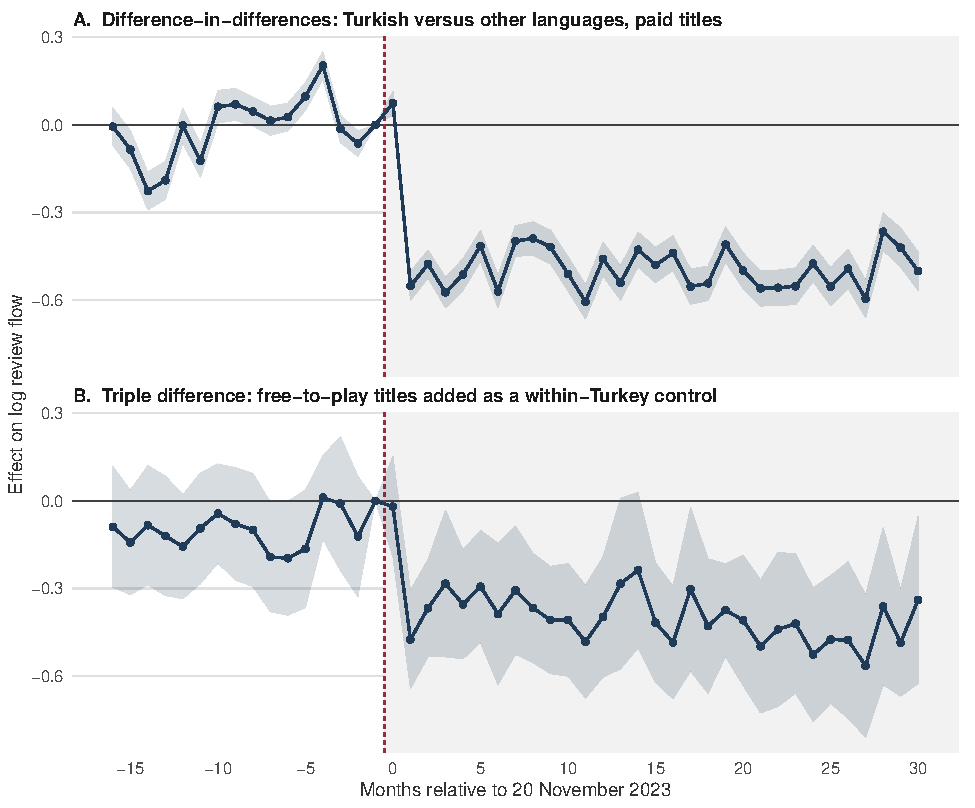
\includegraphics[width=0.86\textwidth]{fig1_event_study.pdf}
\caption{Effect on Turkish review flow, by month relative to 20 November 2023. Panel A is the
difference-in-differences on paid titles; Panel B is the triple difference adding free-to-play
titles as a within-Turkey control. Reference month is October 2023. Shaded bands are 95\%
confidence intervals from standard errors clustered at game $\times$ language.}
\label{fig:event}
\end{figure}

The pre-period is flat. For sixteen months before the change the coefficients sit on zero with no
trend, which is the assumption the design needs and the first thing a sceptical reader should
check. At $k=0$ the series drops and it does not recover: eighteen months later it remains at
essentially its full post-event level. This is what a permanent price change should look like, and it is
not what a gradual macroeconomic deterioration looks like.

Figure~\ref{fig:raw} shows the same thing without any regression, as three indexed series.

\begin{figure}[htbp]
\centering
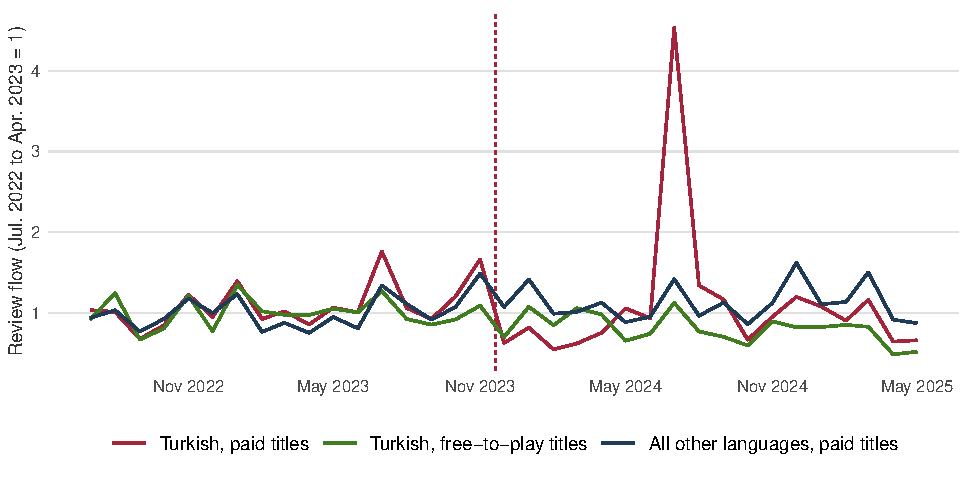
\includegraphics[width=0.86\textwidth]{fig2_raw_flow.pdf}
\caption{Raw review flow, indexed to the July 2022--April 2023 mean. Turkish paid titles, Turkish
free-to-play titles, and paid titles in all other languages. No regression adjustment.}
\label{fig:raw}
\end{figure}

\subsection{Falsification}

\paragraph{Placebo treated languages.} Figure~\ref{fig:ri} relabels each language as treated in
turn. Turkish yields the most negative estimate of all \riN{} languages, and by a wide margin: the
next-most-negative placebo is \riNext{} against Turkish's \bDiD{}. The implied one-sided
randomization-inference $p$-value is \riP{}, which is the smallest value attainable with \riN{}
languages.

\begin{figure}[htbp]
\centering
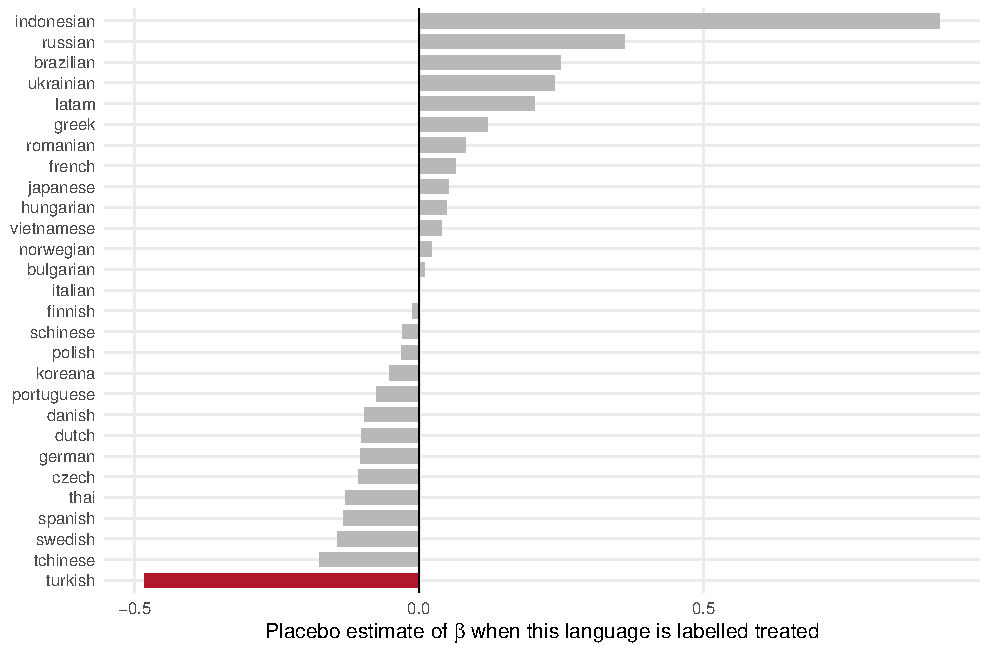
\includegraphics[width=0.80\textwidth]{fig3_ri.pdf}
\caption{Randomization inference. Each bar is the estimated coefficient when that language is
labelled as treated and the specification of column~(1) of Table~\ref{tab:main} is re-estimated.
Turkey, the true treated unit, is shown in red.}
\label{fig:ri}
\end{figure}

The most informative single bar in Figure~\ref{fig:ri} is Russian. Russia experienced a currency
collapse of comparable severity over the same period, and Russian players are subject to the same
platform, the same catalogue, and many of the same macro shocks. The one thing Russia did not
experience is the treatment: Valve retained Ruble pricing, which I confirm holds today. If the
Turkish result were driven by emerging-market currency distress rather than by the price change,
Russian should look like Turkish. It does not.

\paragraph{Placebo dates.} Table~\ref{tab:placebo} re-estimates the specification at false event
dates twelve and six months before, and six months after, the true one. The pre-event placebos are
estimated on the pre-event sample only, so the true change cannot leak into them.

\begin{table}[htbp]
\centering
\caption{Placebo event dates}\label{tab:placebo}
\small
\begin{tabular}{lrrr}
\toprule
Fake event (months from true) & Estimate & Std. error & Obs. \\
\midrule
$-12$ & $0.103$ & ($0.056$) & 4688 \\
$-6$ & $0.097$ & ($0.057$) & 4688 \\
$6$ & $-0.330$ & ($0.060$) & 10255 \\
\midrule
\textbf{True event (0)} & $\mathbf{-0.483}$ & ($\mathbf{0.056}$) & \textbf{10255} \\
\bottomrule
\end{tabular}

\vspace{3pt}
\begin{minipage}{0.86\textwidth}\footnotesize
\emph{Notes.} Each row re-estimates column~(1) of Table~\ref{tab:main} with a false event date the
stated number of months from 20 November 2023. Rows with a negative shift are estimated on
pre-event data only.
\end{minipage}
\end{table}

\paragraph{Leave-one-out.} Dropping each title in turn and re-estimating moves the coefficient only
within $[\looMin, \looMax]$. No single game is responsible.

\section{Mechanisms}\label{sec:mech}

\subsection{Is this a change in demand or a change in who writes reviews?}

This is the paper's central measurement threat, and Table~\ref{tab:composition} addresses it
directly. If Turkish review counts fell because the \emph{type} of Turkish player changed --- if,
say, only the most committed players kept buying and they review at a different rate --- then the
observable characteristics of Turkish reviewers should shift at the event.

\begin{table}[htbp]
\centering
\caption{Reviewer composition and the substitution margin}\label{tab:composition}
\small
\begin{tabular}{lcccc}
\toprule
 & (1) & (2) & (3) & (4) \\
 & Non-Steam key & Share positive & log playtime & log library size \\
\cmidrule(lr){2-5}
Turkish $\times$ Post & $0.0063$ & $-0.0017$ & $0.2752$$^{***}$ & $0.0067$ \\
 & ($0.0061$) & ($0.0036$) & ($0.0399$) & ($0.0613$) \\[3pt]
\midrule
Title $\times$ month FE & Yes & Yes & Yes & Yes \\
Title $\times$ language FE & Yes & Yes & Yes & Yes \\
Observations & 13,724 & 13,724 & 13,724 & 13,724 \\
\bottomrule
\end{tabular}

\vspace{3pt}
\begin{minipage}{0.94\textwidth}\footnotesize
\emph{Notes.} Each column re-estimates the specification of column~(1) of Table~\ref{tab:main}
with a different dependent variable, on paid titles. ``Non-Steam key'' is the share of reviews
from accounts that activated the game from a key not bought on Steam. ``log playtime'' is the log
of median playtime at the time of review. ``log games owned'' is the log of the median library size
of reviewers. Standard errors clustered at game $\times$ language.
\end{minipage}
\end{table}

\subsection{The gray market}

The coefficient on the non-Steam-key share is \bGM{} with a standard error of \seGM. Turkish
buyers did not visibly shift toward third-party key resale. This is a genuine null and I report it
as one; it is also a bounded one, since gray-market keys are only one of several substitution
margins and the most important --- outright piracy --- is unobservable here.

\subsection{Substitution toward free-to-play}

The single most suggestive pattern in the raw data is that Turkish engagement with free-to-play
titles did not fall when paid titles collapsed. In the pilot sample, Turkish review flow for the
free-to-play titles in the panel is flat to rising over the same window in which every paid title
declines. That is consistent with substitution within the platform: when the price of paid games
rises by a factor of several, Turkish players do not leave Steam, they move to the part of Steam
that is still free. This is a suggestive result rather than an identified one --- free-to-play
demand has its own dynamics --- but it matters for welfare, because a consumer who substitutes to
a free title loses less surplus than one who exits.

\section{Magnitudes}\label{sec:magnitudes}

Dividing the reduced-form coefficient by the log price change gives an implied own-price
elasticity between \epsLo{} and \epsHi{}, the range corresponding to price increases of 2{,}900\%
and 240\% respectively. Both ends are inelastic, and by a wide margin.

The revenue arithmetic follows immediately. Take the conservative end of the price change --- a
tripling --- and the estimated quantity response. Revenue per title in Turkey moves from $P\cdot Q$
to $3P \cdot 0.57Q = 1.71 \cdot PQ$. At the aggressive end of the price change the multiple is far
larger. On these numbers, ending the deep Turkish discount \emph{raised} revenue, and had done so
persistently eighteen months later.

That result cuts against the premise on which geographic price discrimination in software is
usually defended, and it should be stated carefully. It does not show that regional pricing is
always unprofitable; it shows that in this market, at these prices, the discount was deeper than
revenue maximisation required. Nor does it settle the welfare question, which points the other
way: an inelastic demand curve means a price increase transfers a large amount of surplus from
consumers to the seller while destroying comparatively little of it. If one cares about the
consumers in question --- players in a country whose median income is a fraction of the American
--- the finding that they kept buying is not reassuring. It is the definition of incidence falling
on them.

Three caveats bound all of this. The elasticity is a chord between two points on a demand curve,
not a slope, so it cannot be extrapolated to smaller price changes. The horizon is eighteen months,
and the long-run response of a games ecosystem to pricing out a national market --- fewer new
players entering, fewer localisations commissioned, a thinner community --- could be considerably
larger than the medium-run one measured here. And the estimate rests on a demand proxy whose
validity Section~\ref{sec:mech} tests but cannot prove.

\section{Conclusion}\label{sec:conclusion}

Valve raised the price of games in Turkey by between roughly 240\% and 2{,}900\% on a single day in
November 2023, for reasons that had nothing to do with the games. Turkish demand for paid titles
fell by about \pctDiD{}\%, and stayed there. Demand for free-to-play titles, in the same country
and the same month, did not move. The implied elasticity is inelastic.

The finding matters beyond video games because the decision Valve made is the decision every firm
selling software internationally makes continuously and quietly. If demand in low-income markets
is as inelastic as this event suggests, then the industry's regional discounts are larger than
profit maximisation requires, and the case for them is distributional rather than commercial ---
which is a very different argument, and one that has to be made explicitly rather than assumed.

Three things would change what can be claimed here, and I do not have any of them.

\emph{Per-title historical prices.} Equation~\eqref{eq:dose} converts this paper's reduced form
into a directly estimated elasticity with a dose-response curve, and requires lira prices
immediately before the change. Recovering them from a licensed price archive would turn a range
into an estimate.

\emph{Units.} Every quantity in this paper is a review. A licensed sales panel would calibrate the
proxy and convert the results into dollars, which is what a welfare calculation needs.

\emph{Argentina.} Argentina was treated on the same day and would double the treated sample, but
Steam's language tags pool Argentine players with the rest of Spanish-speaking Latin America ---
whose countries moved onto a \emph{discounted} dollar price set on that same date, in the opposite
direction. Separating them requires user-level country identification at a scale that raises
collection and ethics questions I am not in a position to resolve alone.

Finally, the most policy-relevant margin in this setting is the one I cannot see at all. When a
game's price in a poor country rises tenfold, some buyers exit, some substitute to free titles ---
and some pirate. I can measure the first two. The third is where the welfare accounting is
decided, and it is open.

\newpage
\begin{thebibliography}{99}\small

\bibitem[Bertrand et al.(2004)]{bertrand2004} Bertrand, M., E. Duflo, and S. Mullainathan (2004).
``How Much Should We Trust Differences-in-Differences Estimates?'' \emph{Quarterly Journal of
Economics} 119(1), 249--275.

\bibitem[Borusyak et al.(2024)]{bjs2024} Borusyak, K., X. Jaravel, and J. Spiess (2024).
``Revisiting Event-Study Designs: Robust and Efficient Estimation.'' \emph{Review of Economic
Studies} 91(6), 3253--3285.

\bibitem[Callaway and Sant'Anna(2021)]{callaway2021} Callaway, B. and P. H. C. Sant'Anna (2021).
``Difference-in-Differences with Multiple Time Periods.'' \emph{Journal of Econometrics} 225(2),
200--230.

\bibitem[Cameron et al.(2008)]{cameron2008} Cameron, A. C., J. B. Gelbach, and D. L. Miller (2008).
``Bootstrap-Based Improvements for Inference with Clustered Errors.'' \emph{Review of Economics and
Statistics} 90(3), 414--427.

\bibitem[Cavallo(2017)]{cavallo2017} Cavallo, A. (2017). ``Are Online and Offline Prices Similar?
Evidence from Large Multi-channel Retailers.'' \emph{American Economic Review} 107(1), 283--303.

\bibitem[Cavallo et al.(2014)]{cavallo2014} Cavallo, A., B. Neiman, and R. Rigobon (2014).
``Currency Unions, Product Introductions, and the Real Exchange Rate.'' \emph{Quarterly Journal of
Economics} 129(2), 529--595.

\bibitem[Choi(2025)]{choi2025} Choi, J. (2025). ``What Happens to App Prices when Developers Pay
Lower Commission Fees? Evidence from the European Union.'' November. Study for which support was
provided by Apple. Available at \url{https://developer.apple.com/download/files/DMA-Study-Nov-2025.pdf}.

\bibitem[Conley and Taber(2011)]{conley2011} Conley, T. G. and C. R. Taber (2011). ``Inference with
`Difference in Differences' with a Small Number of Policy Changes.'' \emph{Review of Economics and
Statistics} 93(1), 113--125.

\bibitem[Danaher et al.(2010)]{danaher2010} Danaher, B., S. Dhanasobhon, M. D. Smith, and R. Telang
(2010). ``Converting Pirates without Cannibalizing Purchasers: The Impact of Digital Distribution
on Physical Sales and Internet Piracy.'' \emph{Marketing Science} 29(6), 1138--1151.

\bibitem[Danaher et al.(2014)]{danaher2014} Danaher, B., M. D. Smith, and R. Telang (2014).
``Piracy and Copyright Enforcement Mechanisms.'' \emph{Innovation Policy and the Economy} 14,
25--61. NBER Working Paper 19150.

\bibitem[Goodman-Bacon(2021)]{goodmanbacon2021} Goodman-Bacon, A. (2021).
``Difference-in-Differences with Variation in Treatment Timing.'' \emph{Journal of Econometrics}
225(2), 254--277.

\bibitem[Gorodnichenko and Talavera(2017)]{gorodnichenko2017} Gorodnichenko, Y. and O. Talavera
(2017). ``Price Setting in Online Markets: Basic Facts, International Comparisons, and Cross-Border
Integration.'' \emph{American Economic Review} 107(1), 249--282.

\bibitem[Howell and Parker(2024)]{howellparker2024} Howell, S. T. and D. Parker (2024). ``VC Funds
and Regulation D's Rule 506(c): Did Permitting General Solicitation Open the Door for Emerging and
Underrepresented Managers?'' Report prepared under contract with the SEC Office of the Advocate for
Small Business Capital Formation, October.

\bibitem[Silva and Tenreyro(2006)]{silva2006} Santos Silva, J. M. C. and S. Tenreyro (2006). ``The
Log of Gravity.'' \emph{Review of Economics and Statistics} 88(4), 641--658.

\bibitem[Sun and Abraham(2021)]{sunabraham2021} Sun, L. and S. Abraham (2021). ``Estimating Dynamic
Treatment Effects in Event Studies with Heterogeneous Treatment Effects.'' \emph{Journal of
Econometrics} 225(2), 175--199.

\bibitem[Tud\'on(2022)]{tudon2022} Tud\'on, J. (2022). ``Distilling Network Effects from Steam.''
\emph{Quantitative Marketing and Economics}. DOI 10.1007/s11129-022-09254-5.

\bibitem[Watabe et al.(2025)]{watabe2025} Watabe, Y., H. Yang, and E. Kanasheuski (2025). ``Can
Digital Distribution Defy the Law of Gravity?'' \emph{Canadian Journal of Economics} 58(3),
1123--1146.

\bibitem[Young(2019)]{young2019} Young, A. (2019). ``Channeling Fisher: Randomization Tests and the
Statistical Insignificance of Seemingly Significant Experimental Results.'' \emph{Quarterly Journal
of Economics} 134(2), 557--598.

\end{thebibliography}

\end{document}
